\documentclass{beamer}

\usetheme{Singapore}
\usecolortheme{seahorse}
\usefonttheme{structuresmallcapsserif}

\usepackage[utf8]{inputenc}
\usepackage[english]{babel}

\usepackage{default}

\usepackage{hyperref}

\usepackage{multicol}

\newcommand{\pfeil}{$\rightarrow $ }

	\title[PAC]{Presentation-Abstraction-Control} 
	%\subtitle[Optionaler Subtitle]{Optionaler Subtitle des sehr langen Titels der Präsentation}
	\author[Grn. HI]{Gruppen H und I} 
	\institute[SE]{Software Engineering WS 17/18}
	\date{\today}
	
	
	
%TODO Notes aus für Endversion
\setbeameroption{show notes}

\begin{document}

\begin{frame}[plain,noframenumbering]  %Keine Fußzeile auf erster Seite und keine Nummerierung
	\titlepage
\end{frame}



\section{Example}

\section{Context}

\section{Problem}
%Ann-Kathrin

\begin{frame}
\frametitle{Problem}

%Bild noch rein?


\begin{multicols}{2}
 


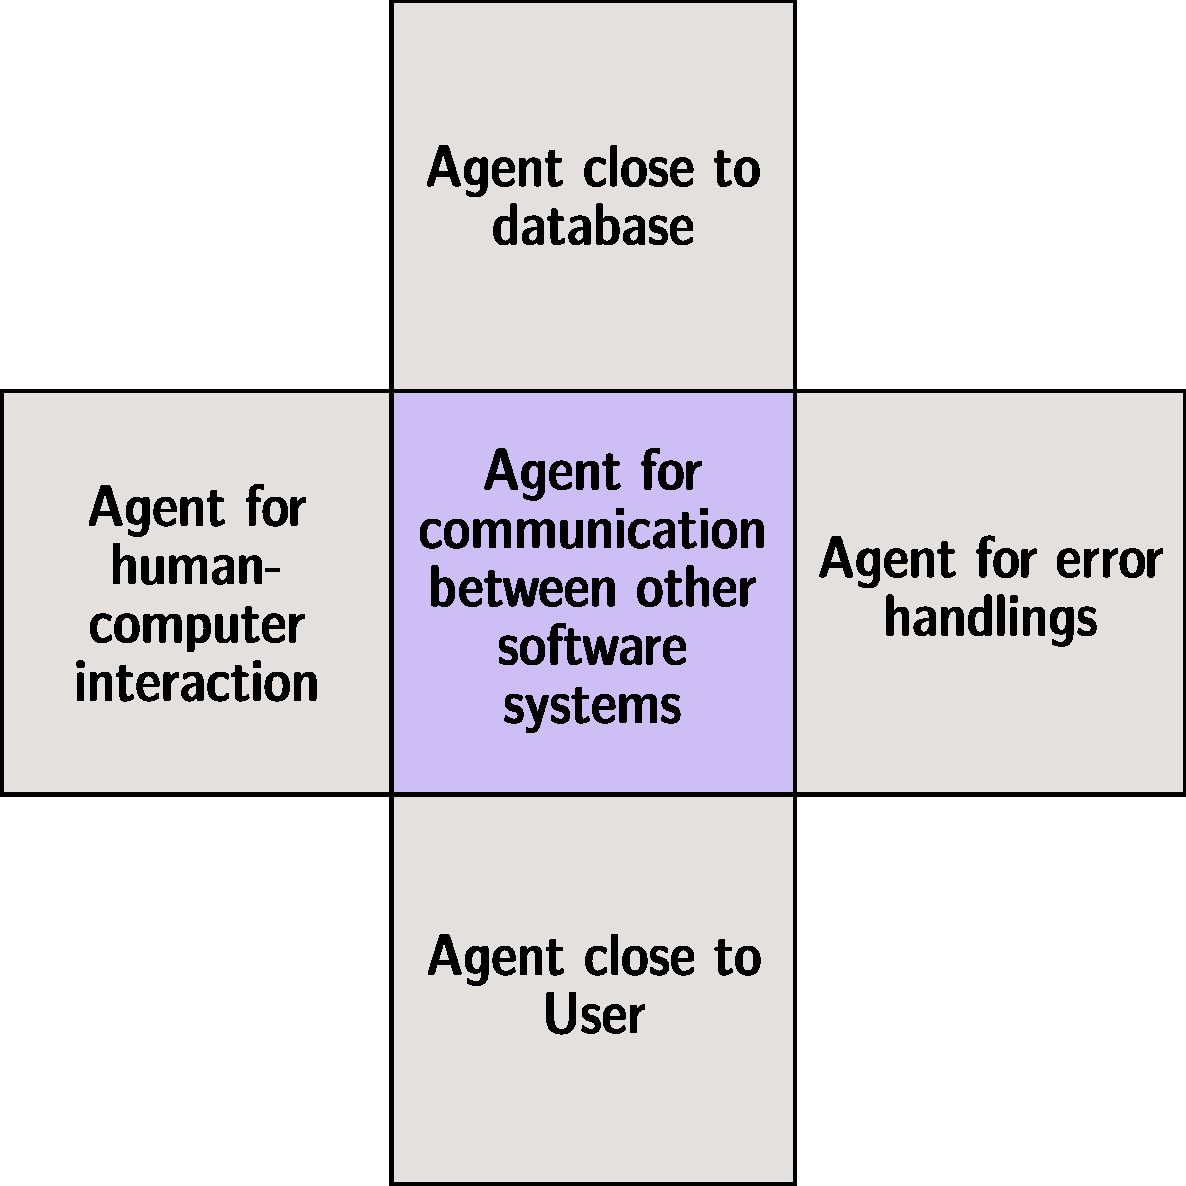
\includegraphics[width=0.4\textwidth]{./pics/problem.pdf}
% problem.pdf: 0x0 pixel, 300dpi, 0.00x0.00 cm, bb=


There are three main Problems based on that:

 \begin{itemize}
  \item Agents often maintain their own state and data
  \item Interactive agents provide their own user interface
  \item Systems evolve over time
 \end{itemize}
\end{multicols}

\note{Ann-Kathrin}


\end{frame}


\section{Solution}

\begin{frame}
\frametitle{Solution}

\begin{center}
 \includegraphics[width=0.7\textwidth]{./pics/solution.eps}
 % solution.eps: 0x0 pixel, 300dpi, 0.00x0.00 cm, bb=0 -1 744 237
\end{center}


 \begin{itemize}
  \item Tree-like hierarchy of PAC agents
  \item PAC agents consist of:
  \begin{itemize}
   \item \textbf{Presentation} component (visible behavior)
   \item \textbf{Abstraction} component (data model with its functional operations)
   \item \textbf{Control} component (connects data model and view; provides communication
between other agents)
  \end{itemize}
 \end{itemize}

 \note{Lucas}
 
\end{frame}


\section{Structure}

\begin{frame}
 \frametitle{Structure}
 
 \note{Nicole, Jaqueline}
\end{frame}


\subsection{Top-Level Agent}

\begin{frame}
 \frametitle{Top-Level Agent}
 
 \note{Nicole, Jaqueline}
\end{frame}

\subsection{Bottom-Level Agent}

\begin{frame}
 \frametitle{Bottom-Level Agent}
 
 \begin{itemize}

  \item Presentation component
  \begin{itemize}
   \item specific view on the object
    \item provides access to functions
    \item maintains information
  \end{itemize}
  \item Abstraction component
  \begin{itemize}
    \item maintains agent-specific data
  \end{itemize}
  \item Control component
  \begin{itemize}
   \item manages relation between abstraction and presentation component
    \item communication to intermediate agents
  \end{itemize}

 \end{itemize}


 
 \note{Vera}
\end{frame}

\subsection{Intermediate-Level Agent}


\begin{frame}
 \frametitle{Intermediate-Level Agent}
 
 Responsibility:
 
 \begin{itemize}
  \item coordinate lower-level PAC agents
  \item Composes lower-level PAC agents to a single unit of higher abstractation
 \end{itemize}
 

 \note{Anna \\
 Kann raus bei Platzmangel}
\end{frame}

\begin{frame}
 \frametitle{Intermediate-Level Agent}
 
 \begin{center}
 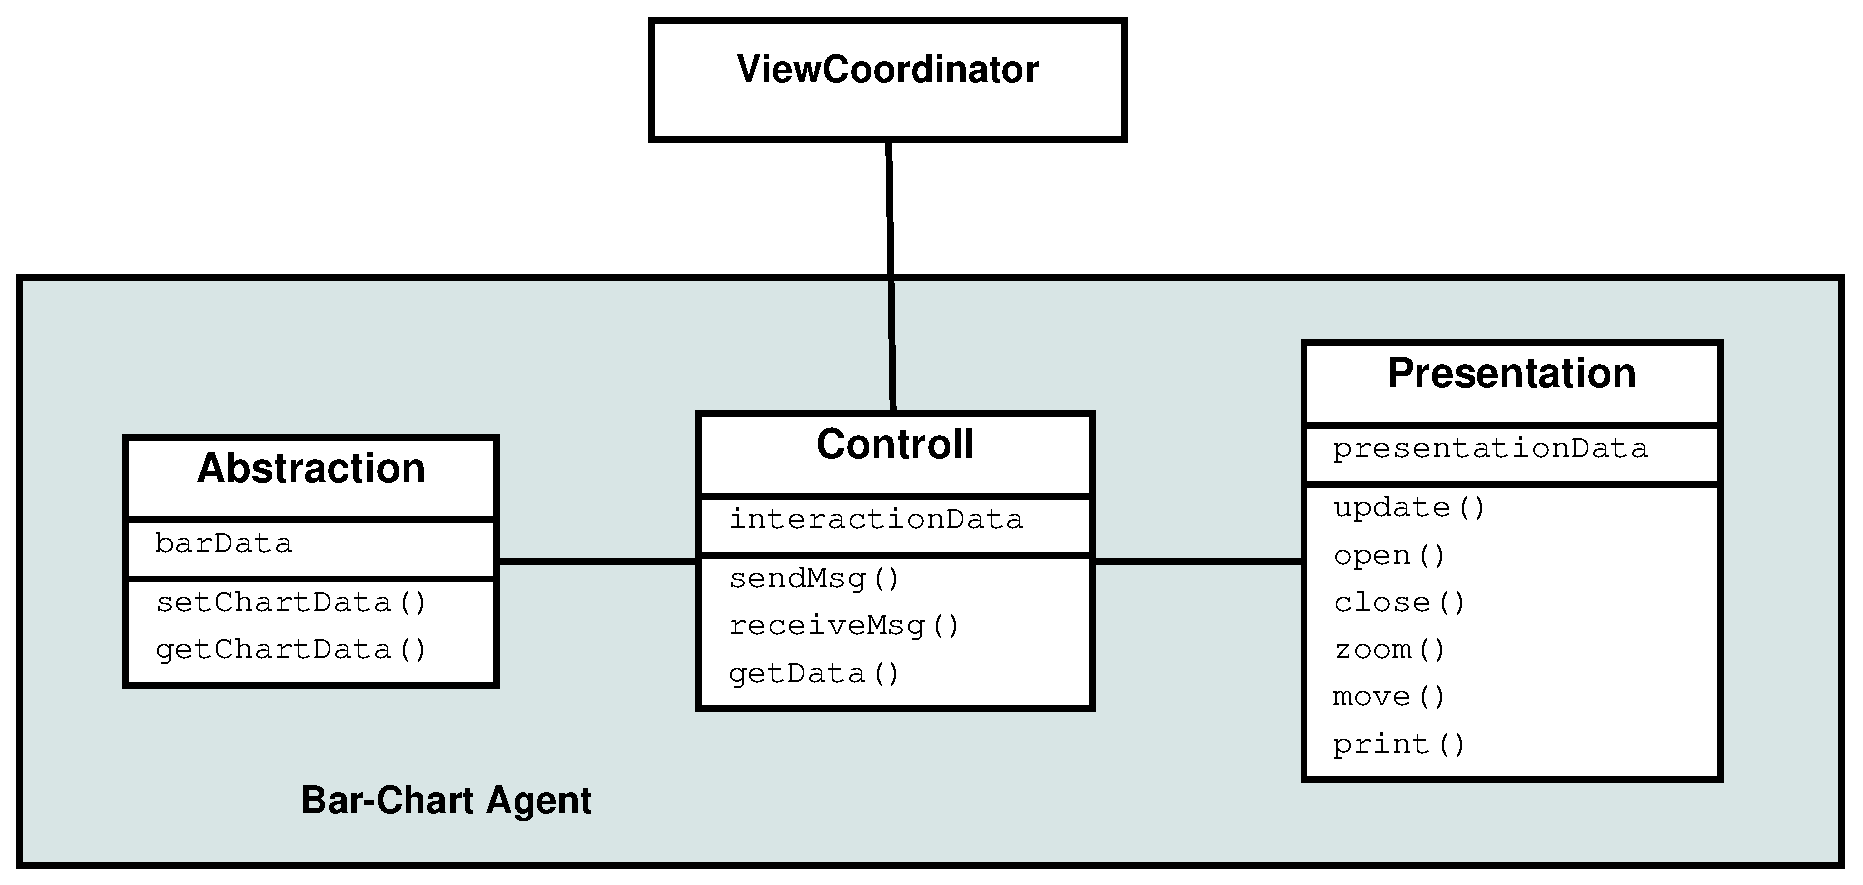
\includegraphics[width=.8\textwidth]{./pics/Components.eps}
 % Components.eps: 0x0 pixel, 300dpi, 0.00x0.00 cm, bb=0 0 878 409
\end{center}

 
 \begin{itemize}
  \item abstract component manages the data
  \item presentation component implements user interface 
  \item control component communicates with top-level and bottom-level agents

%TODO Text kürzen

 \end{itemize}
 
 \note{Anna\\
 gekürzt, lange Version: \\
  \begin{itemize}
  \item abstract component manages the data
\pfeil responsible for all currently active views
  \item presentation component implements user interface 
\pfeil creates a tool to view the election data for example in bar or pie charts
  \item control component communicates with top-level and bottom-level agents
\pfeil control all subordinate agents



 \end{itemize}
 }

\end{frame}


 

\section{Dynamics}

\begin{frame}
 \frametitle{Dynamics}
 Bild 1
 
 %TODO Bild 1 erstellen / einfügen
 
 \note{Nicole}
\end{frame}

\begin{frame}
 \frametitle{Dynamics}
 Bild 2
 
 %TODO Bild 2 erstellen / einfügen
 
 \note{Nicole}
\end{frame}

\section{Known Uses}

\begin{frame}
 \frametitle{Known Issues}
 
 \note{Fabian}
\end{frame}

\begin{frame}
 \frametitle{Quellen}

 %TODO Quellen hinzufügen
 
 \note{Rebecca}
\end{frame}






\end{document}
